\def\theTopic{Reading 18}

\begin{center}
{\bf {\large Data Distribution versus Sampling Distribution }}
\end{center}


For the SAT,  ACT, and baby weight examples, we assumed that the
individual data points have a normal distribution.   We said that the
score of one individual test taker or the weight of one baby follows a
normal distribution.  Think of picking one value at random from one of
these distributions:



% par(mfrow=c(1,3))
% curve(dnorm(x, 21,5), 6, 36, xlab = "ACT", bty="l", yaxt="n", ylab = " ")
% curve(dnorm(x, 1500,300), 400, 2400, xlab = "SAT", bty="l", yaxt="n", ylab = " ")
% curve(dnorm(x, 3000,700), 900, 5100, xlab = "Baby Weights", bty="l", yaxt="n", ylab = " ")
% dev.copy(png, "plots/3normals.png", height = 200, width = 600);dev.off()

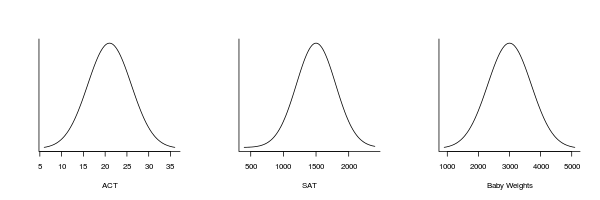
\includegraphics[width=\linewidth]{plots/3normals.png}

Values near the centers of the curves are more likely to get picked
that values out in the tails. 



Another important use of distributions is the {\bf sampling
  distribution} of a {\bf statistic}.  We have already been using sampling
distributions, but have simulated draws to get them and have drawn
them as dot plots.  We'll see in the next lesson that the sampling
distribution of a proportion often is well approximated by a normal
distribution. Before we get there, though, we want to insert a
reminder about just what a sampling distribution is.

The {\bf sampling distribution} of a {\bf statistic} is a description
of all the possible values that statistic can take and the probability
of each.  For example, if we randomly sample weights of 9 full term
babies, each coming from N(3000,700), the sample mean will also be
normally distributed with mean 3000, but the standard deviation will
be 233g instead of 700g.  Think about the sampling distribution this
way: 
\begin{itemize}
\item When we randomly sample and compute a statistic from the sample,
  we don't know what we'll get ahead of time for any one draw, and
  won't know what mean we will get.  The mean ($\xb$) is, then, a random
  variable.
\item We do know quite a bit about the distribution of $\xb$. Because
  the distribution of the individual data points is normal, so is the
  distribution of $\xb$. \\
  Averaging values together does not change the
  center, so the center of the distribution of $\xb$ is also 3000g.  \\
  Averaging pulls in extremes, and the spread of the sampling
  distribution becomes $700/\sqrt{9} = 233.3$g.
\end{itemize}\vspace{1in}



\begin{center}
  {\large\bf Important Points}
\end{center}

\begin{itemize}
\item  It is important to distiguish between the sampling distribution
  of a statistic and the underlying distribution of individual data
  points.  
\item If we start with a normal distribution for individual points,
  then the sample mean will also have a normal distribution with the
  same center.
\item As sample size increases, spread decreases: the standard
  deviation of $\xb$ is  $\frac{\sigma}{\sqrt{n}}$. 
\end{itemize}

